\maketitle

\cleardoublepage
\phantomsection
\addcontentsline{toc}{chapter}{Indice}
\tableofcontents

\listoffigures

\chapter{Introduzione}
\textsl{\textbf{Climate Monitoring}} è un'applicazione sviluppata nell’ambito del progetto di Laboratorio Interdisciplinare B (A.A. 2023/24) per il corso di laurea in Informatica dell’\textsl{Universit\`a degli Studi dell’Insubria} di Varese.

Il progetto è sviluppato in \textsl{Java 17} sui sistemi operativi \textsl{Arch Linux} e \textsl{Windows 11}.
L'applicazione è stata testata sugli stessi sistemi.

Questo manuale descrive la struttura del progetto e delle risorse che utilizza. Per avere informazioni più dettagliate consultare la JavaDoc del codice sorgente.

\section{Librerie in Comune al Client e al Server Utilizzate}

Per lo sviluppo di questo progetto sono state utilizzate alcune librerie di terze parti.

Per le librerie specifiche al client (Capitolo \ref{ch:client}) e al server (Capitolo \ref{ch:server}) riferirsi ai capitoli appropriati.

\subsection{\textsl{Lombok}}

\href{https://projectlombok.org/}{Link al sito del progetto}

Il progetto Lombok mira a ridurre la quantità di codice scritto tramite annotazioni che si attivano a tempo di compilazione. Si è scelto di utilizzarlo in modo da ottimizzare la stesura del codice.

\subsection{\textsl{Apache Log4j}}

\href{https://logging.apache.org/log4j/2.x/}{Link al sito del progetto}

Si è scelto di usare \textsl{Log4j} come sostegno al progetto per via della sua popolarità e comprovata robustezza.

\chapter{Architettura della soluzione sviluppata}
Il sistema (senza considerare il database) è stato sviluppato in tre moduli principali:
\begin{itemize}
	\item \texttt{org.a3b.clientCM}
	\item \texttt{org.a3b.serverCM}
	\item \texttt{org.a3b.commons}
\end{itemize}

\begin{figure}[h]
	\centering
	\caption{Architettura modulare di sistema}
	\label{fig:architettuta}
	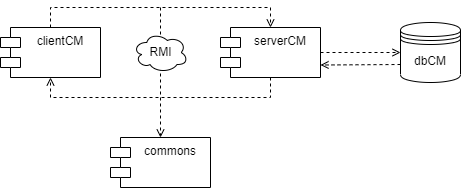
\includegraphics[width=0.8\linewidth]{../../fig/img/tecnico/architettuta.drawio}
\end{figure}

Client e server comunicano tra di loro tramite RMI. Le risorse di sistema utili ad entrambi i suddetti moduli sono contenute in \texttt{org.a3b.commons}.

Il database PostgreSQL comunica con il server per fornire e ricevere dati.

\pagebreak
Il funzionamento generale dell'applicazione è illustrato nel seguente diagramma:

\begin{figure}[h]
	\centering
	\caption{Sequence diagram per illustrare il funzionamento generale del sistema}
	\label{fig:sequence}
	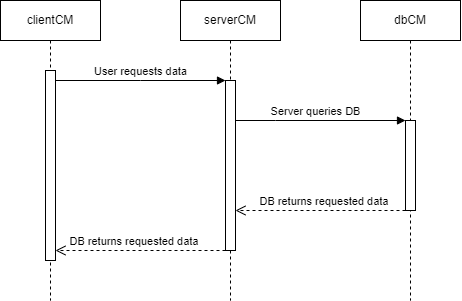
\includegraphics[width=0.7\linewidth]{../../fig/img/tecnico/sequence.drawio}
\end{figure}

\chapter{Database (dbCM)}
\label{ch:db}
Di seguito si mostra lo schema Entità-Relazione del database di supporto all’esecuzione dei servizi della piattaforma Climate Monitoring.

\begin{figure}[h]
	\centering
	\caption{Schema ER del database}
	\label{fig:erdb}
	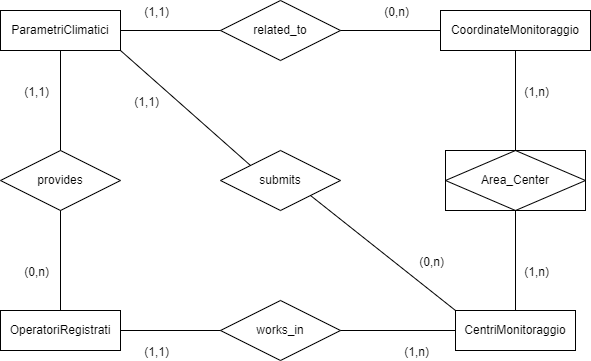
\includegraphics[width=0.8\linewidth]{../../fig/img/tecnico/ERdb.drawio}
\end{figure}

In questo schema vengono illustrate le entità richieste dalle specifiche e le relative associazioni.

Nel dettaglio:
\begin{itemize}
	\item \textbf{\textit{CentriMonitoraggio}}, contenente tutte le informazioni relative ai centri di monitoraggio registrati nel sistema, creati dai vari operatori;
	\item \textbf{\textit{CoordinateMonitoraggio}}, contenente i dati riguardanti le aree geografiche presenti nel documento \textit{"CoordinateMonitoraggio.xlsx"} fornito nelle specifiche di progetto;
	\item \textbf{\textit{OperatoriRegistrati}}, racchiude i dettagli relativi gli operatori che hanno effettuato la registrazione al sistema;
	\item \textbf{\textit{ParametriClimatici}}, modella dei record per racchiudere le informazioni che interessano le misurazioni effettuate in determinate aree d'interesse dagli operatori registrati, per conto dei relativi centri di monitoraggio.
\end{itemize}
\pagebreak
Le associazioni costruite sulle entità appena elencate sono le seguenti:
\begin{itemize}
	\item \textbf{\textit{"provides"}}, tra \textit{OperatoriRegistati} e \textit{ParametriClimatici}, con cardinalità \textbf{\textit{(0,n)-(1,1)}}
	      
	      Ogni operatore registrato può difatti fornire più misurazioni climatiche, mentre una misurazione può essere stata fornita da uno e un solo operatore registrato.
	\item \textbf{\textit{"related\_to"}}, tra \textit{ParametriClimatici} e \textit{CoordinateMonitoraggio}, con cardinalità \textbf{\textit{(1,1)-(0,n)}}
	      
	      Ogni misurazione climatica deve difatti essere relativa a una e una sola area geografica, mentre un'area geografica può avere associate molteplici misurazioni, come non averne.
	\item \textbf{\textit{"submits"}}, tra \textit{CentriMonitoraggio} e \textit{ParametriClimatici}, con cardinalità \textbf{\textit{(0,n)-(1,1)}}
	      
	      Ogni centro di monitoraggio può presentare più misurazioni relative alle proprie aree d'interesse, mentre una misrurazione deve essere stata resa disponibile da uno e un solo centro di monitoraggio.
	\item \textbf{\textit{"works\_in"}}, tra \textit{OperatoriRegistrati} e \textit{CentriMonitoraggio}, con cardinalità \textbf{\textit{(1,1)-(1,n)}}
	      
	      Ogni operatore deve associarsi a un centro di monitoraggio in seguito alla registrazione, se quello a cui vuole associarsi non è presente nel sistema, ne crea uno nuovo. In ogni centro di monitoraggio lavora almeno un operatore (il suo creatore), ed eventualmente altri associati.
	\item \textbf{\textit{"Area\_Center"}}, tra \textit{CoordinateMonitoraggio} e \textit{CentriMonitoraggio}, con cardinalità \textbf{\textit{(1,n)-(1,n)}}
	      
	      Ogni area geografica può essere considerata d'interesse da più centri di monitoraggio, i quali a loro volta possono monitorare molteplici aree d'interesse.
	      Sulla base di questa associazione, in seguito alla ristrutturazione dello schema ER è stata costruita un'ulteriore relazione omonima, trattandosi di un'associazione di tipo "molti a molti".
\end{itemize}
Escludendo quest'ultima, le prime quattro associazioni mostrate (trattandosi di assocazioni di tipo "uno a molti"/"molti a uno") sono state invece riportate nello schema relazionale come vincoli di chiave esterna.
\pagebreak

Il seguente schema relazionale mostra nel dettaglio gli attributi (con i vari tipi associati) di ogni relazione e i relativi vincoli di chiave primaria ed esterna.

\begin{figure}[h]
	\centering
	\caption{Schema dettagliato del database}
	\label{fig:quickdbd-clima}
	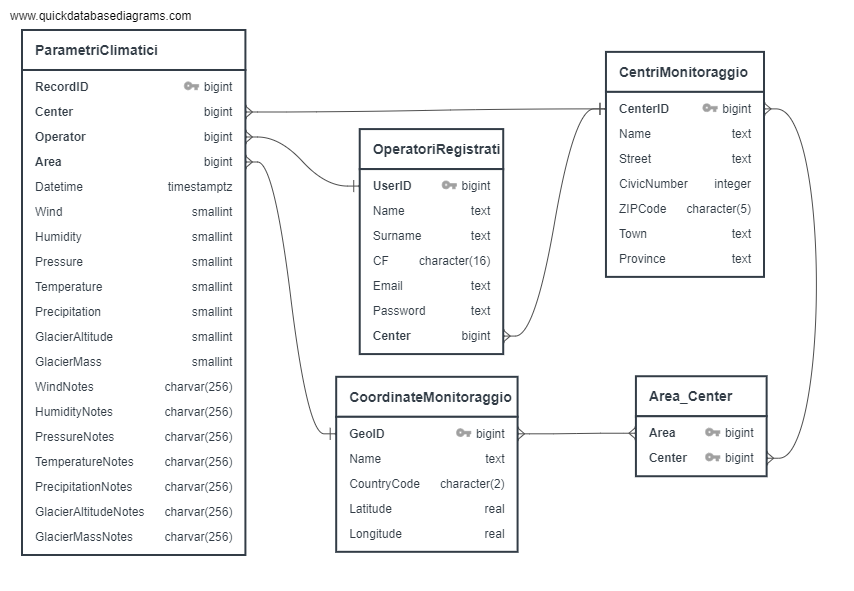
\includegraphics[width=0.8\linewidth]{../../fig/img/tecnico/QuickDBD-clima}
\end{figure}

Gli attributi di ogni relazione sono stati inseriti sulla base delle indicazioni fornite nel documento delle specifiche di progetto. Al riguardo, sono degne di nota le seguenti scelte progettuali:
\begin{itemize}
	\item in \textit{\textbf{ParametriClimatici}}, è stato aggiunto l'attributo \textit{"RecordID"}, utilizzato come chiave primaria della relazione, in modo da usufruire di un identificatore univoco per ogni record che riguarda le misurazioni climatiche; inoltre gli attributi riguardanti le note dei parametri di rilevazione non sono stati dichiarati \textit{"NULLABLE"}, in quanto l'eventuale mancanza di tali dati (opzionali) è stata gestita a livello applicativo tramite l'uso di stringhe vuote;
	\item in \textit{\textbf{CoordinateMonitoraggio}}, gli attributi \textit{"Latitude"} e \textit{"Longitude"} sono stati separati, nonostante nel documento \textit{"CoordinateMonitoraggio.xlsx"} (fornito nelle specifiche di progetto, sulla base del quale è stata costruita questa relazione) siano parte dello stesso campo \textit{"Coordinates"}, in modo da facilitarne la manipolazione a livello applicativo.
\end{itemize}

\section{JDBC}
Per l'integrazione del linguaggio SQL necessario per la gestione e manipolazione dei dati all'interno del database è stata utilizzata l'interfaccia JDBC (Java Database Connectivity), come richiesto nei requisiti del progetto.

\chapter{Modulo \texttt{org.a3b.clientCM}}
\label{ch:client}
Il modulo clientCM gestisce il lato client dell'applicazione. Per ulteriori informazioni consultare il codice sorgente.

\begin{figure}[h]
	\centering
	\caption{Struttura del modulo clientCM}
	\label{fig:clientcm}
	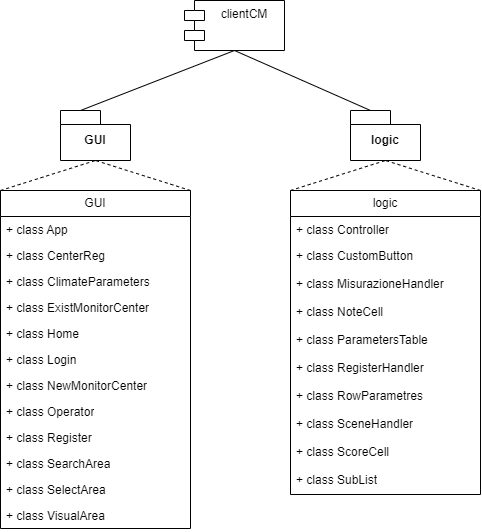
\includegraphics[width=0.7\linewidth]{../../fig/img/tecnico/clientCM.drawio}
\end{figure}

\pagebreak
Come si può notare dal diagramma, comprende due package:
\begin{itemize}
	\item \texttt{GUI}, per raccogliere il codice dedicato allo sviluppo dell'interfaccia grafica, in particolare:
	\begin{itemize}
		\item \texttt{App}, contiene lo start dell'applicazione;
		\item \texttt{CenterReg}, gestisce la registrazione dei centri di monitoraggio;
		\item \texttt{ClimateParameters}, gestisce l'inserimento dei parametri climatici;
		\item \texttt{ExistMonitorCenter}, gestisce la visualizzazione dei centri di monitoraggio presenti nel sistema;
		\item \texttt{Home}, gestisce la visualizzazione della schemata iniziale;
		\item \texttt{Login}, gestisce la schermata del login all'applicazione;
		\item \texttt{NewMonitorCenter}, gestisce la creazione di nuovi centri di monitoraggio;
		\item \texttt{Operator}, gestisce le funzioni che un operatore registrato al sistema può svolgere;
		\item \texttt{Register}, gestisce la registrazione degli operatori al sistema;
		\item \texttt{SearchArea}, gestisce la ricerca delle aree geografiche;
		\item \texttt{SelectArea}, gestisce la selezione di aree geografiche in modo da poterle inserire nella lista di aree d'interesse di un centro di monitoraggio;
		\item \texttt{VisualArea}, gestisce la visualizzazione dei parametri climatici inseriti relativi a una determinata area geografica;
	\end{itemize}
	\item \texttt{logic}, contenente la logica applicativa del lato client del sistema, in particolare:
	\begin{itemize}
		\item \texttt{Controller}, gestisce i controlli relativi ai parametri inseriti dall'utente;
		\item \texttt{CustomButton}, modella i pulsanti "\textit{back}" e "\textit{home}";
		\item \texttt{MisurazioneHandler}, gestisce la visualizzazione e l'inserimento di parametri climatici all'interno del sistema;
		\item \texttt{NoteCell}, gestisce l'inserimento delle note associate ai vari parametri climatici;
		\item \texttt{ParametersTable}, gestisce la tabella di inserimento di parametri climatici;
		\item \texttt{RegisterHandler}, gestisce la registrazione degli operatori;
		\item \texttt{RowParametres}, gestisce i singoli dati nella tabella di inserimento parametri climatici;
		\item \texttt{SceneHandler}, gestisce la visualizzazione delle scene generiche;
		\item \texttt{ScoreCall}, gestisce i punteggi assegnati a ogni parametro climatico;
		\item \texttt{SubList}, gestisce la selezione dei centri di monitoraggio;
	\end{itemize}
\end{itemize}

\section{Librerie Utilizzate dal Client}
Per lo sviluppo dell'interfaccia grafica è stata utilizzata in particolare la seguente libreria:

\subsection{\textsl{Open JavaFX}}
\label{ch:javafx}

\href{https://openjfx.io/}{Sito del progetto}

Libreria per costruzione di interfacce grafiche in Java.

\chapter{Modulo \texttt{org.a3b.serverCM}}
Il modulo serverCM gestisce il lato server dell'applicazione. Per ulteriori informazioni consultare il codice sorgente.
\label{ch:server}

\begin{figure}[h]
	\centering
	\caption{Struttura del modulo serverCM}
	\label{fig:severcm}
	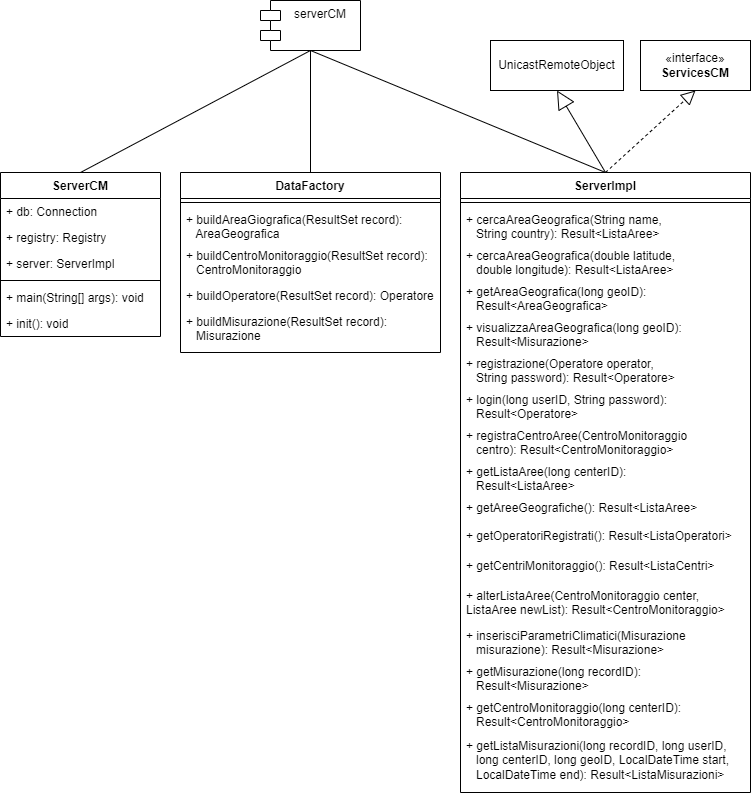
\includegraphics[width=0.9\linewidth]{../../fig/img/tecnico/serverCM.drawio}
\end{figure}
\pagebreak

Come si può notare dal diagramma, comprende:
\begin{itemize}
	\item classe \textbf{\texttt{ServerCM}}
		
		Si occupa della connessione RMI per rendere il sistema distribuito e della connessione con il database;
	\item classe \textbf{\texttt{DataFactory}}
		
		Contiene metodi che permettono di creare le varie istanze d'interesse a partire da record estratti dal database;
	\item classe \textbf{\texttt{ServerImpl}}
		
		Implementazione vera e propria del server, estende \texttt{UnicastRemoteObject} (per essere inserita nel registry di RMI) e implementa l'interfaccia \texttt{ServicesCM}, che contenente tutte le funzioni richieste (Capitolo \ref{ch:commons}).
\end{itemize}

\section{Librerie Utilizzate dal Server}

\subsection{Dalla Libreria Standard di Java}

\begin{itemize}
	\item \texttt{java.rmi}, per rendere il sistema distribuito;
	\item \texttt{java.sql}, per supportare le operazioni che coinvolgono il database;
	\item \texttt{java.util};
\end{itemize}


\subsection{\textsl{PostgreSQL JDBC Driver}}

\href{https://mvnrepository.com/artifact/org.postgresql/postgresql/42.7.3}{Maven Central}

Driver JDBC per connettere il server al database PostgreSQL.

\subsection{\textsl{dotenv-java}}

\href{https://mvnrepository.com/artifact/io.github.cdimascio/dotenv-java/3.0.0}{Maven Central}
	
Libreria adibita alla lettura di file \texttt{.env}.

\chapter{Modulo \texttt{org.a3b.commons}}
\label{ch:commons}
Commons contiene e gestisce l'insieme di risorse utilizzate sia dal modulo clientCM che da serverCM.

\begin{figure}[h]
	\centering
	\caption{Struttura del modulo commons}
	\label{fig:commonscm}
	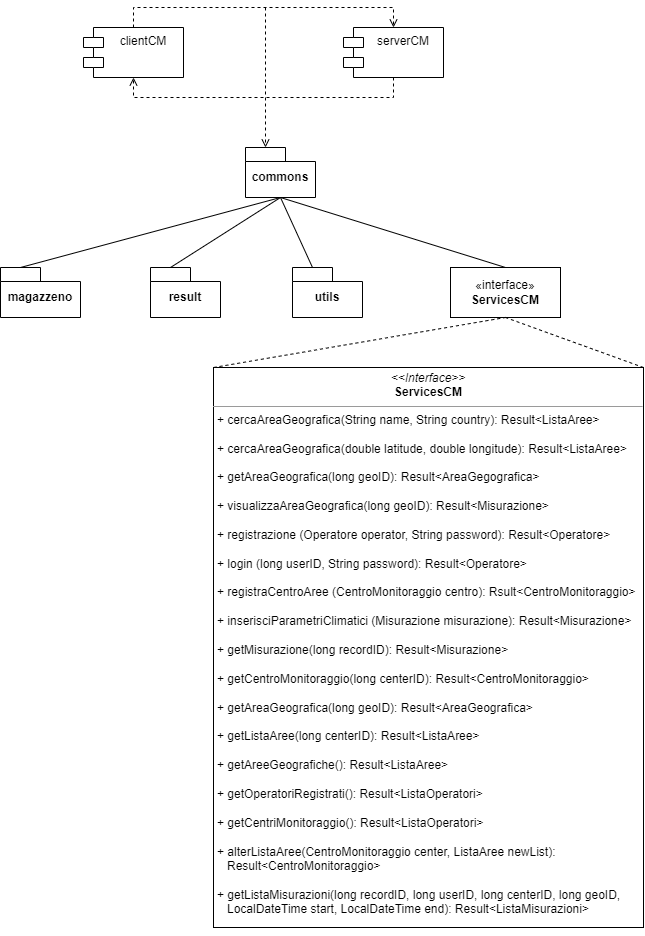
\includegraphics[width=0.7\linewidth]{../../fig/img/tecnico/CM.drawio}
\end{figure}
\pagebreak
Come si può notare dal diagramma, comprende:
\begin{itemize}
	\item package \textbf{\texttt{magazzeno}}
		
		Contiene le classi che modellano le istanze gestite dal sistema, in particolare:
		\begin{itemize}
			\item \texttt{AreaGeografica}, rappresenta un'area di interesse per la rilevazione di parametri climatici;
			\item \texttt{CentroMonitoraggio}, rappresenta un centro di monitoraggio;
			\item \texttt{ListaAree}, rappresenta una lista di aree geografiche presenti nel database;
			\item \texttt{ListaCentri}, rappresenta una lista di centri di monitoraggio presenti nel database;
			\item \texttt{ListaMisurazioni}, rappresenta una lista di misurazioni climatiche presenti nel database;
			\item \texttt{ListaOperatori}, rappresenta una lista di operatori registrati nel database;
			\item \texttt{Misurazione}, rappresenta il risultato di una rilevazione climatica;
			\item \texttt{Operatore}, rappresenta un operatore dei centri di monitoraggio.
		\end{itemize}
	\item package \textbf{\texttt{result}}
		
		Modella un "contenitore" utilizzato per una gestione migliore dei possibili errori generati all'interno dell'applicazione.
		Per ulteriori informazioni consultare i relativi codice sorgente e JavaDoc.
	\item package \textbf{\texttt{utils}}
		
		Contiene elementi che facilitano la lettura e l'organizzazione del codice, in particolare:
		\begin{itemize}
			\item interfaccia \texttt{CercaAree}, per la ricerca di aree geografiche;
			\item interfaccia \texttt{MediaAree}, per il calcolo della media dei valori assegnati ai parametri climatici;
			\item enumerativo \texttt{TipoDatoGeogafico}, modella i vari parametri di ogni rilevazione climatica.
		\end{itemize}
	\item interfaccia \textbf{\texttt{ServicesCM}}
	
		Racchiude tutte i metodi forniti dal server e utilizzate dal client. In particolare sono presenti tutte le funzioni richieste dalle specifiche di progetto.
\end{itemize}

\chapter{Scelte strutturali e algoritmiche rilevanti}
\begin{itemize}
	\item utilizzo di un \texttt{HashMap} per gestire \texttt{Misurazione}
	
	Nella classe \texttt{Misurazione} (Capitolo \ref{ch:commons}) è stata utilizzata la struttra dati \texttt{HashMap} fornita dalla libreria nativa di Java \texttt{java.util}, che associa delle chiavi a determinati valori. In questo caso viene associato un \texttt{TipoDatoGeografico} al proprio valore (da 0 a 5), in modo che quest'ultimo sia relativo al corretto parametro climatico.
	
	\item \texttt{ListaAree}, \texttt{ListaCentri}, \texttt{ListaMisurazioni}, \texttt{ListaOperatori} (Capitolo \ref{ch:commons}) estendono \texttt{ConcurrentLinkedDeque<E>}
	
	Tutte classi che rappresentano una lista di istanze nel sistema estendono \texttt{ConcurrentLinkedDeque<E>} invece che \texttt{LinkedList<E>} in modo da garantire la consistenza dei dati evitando problemi di concorrenza.
	
	\item metodo \texttt{ServerImpl.alterListaAree()}
	
	Il metodo \texttt{alterListaAree()}, che aggiorna la lista di aree associate a un determinato centro di monitoraggio, è strutturato nel seguente modo:
	\begin{enumerate}
		\item dalla tabella del database (dbCM, Capitolo \ref{ch:db}) Area\_Center vengono cancellate tutte le aree geografiche appartenenti alla lista da modificare;
		\item vengono inserite (tramite una seconda query) le aree geografiche appartenenti alla lista modificata.
	\end{enumerate}
	
	Nonostante il metodo a livello logico possa sembrare poco ottimizzato (nel caso la lista da modificare e quella aggiornata differiscano solo per poche istanze, quelle presenti in entrambe verrebbero eliminate e reinserite), è stato scelto di implementarlo nel suddetto modo, in quanto: 
	\begin{itemize}
		\item viene minimizzata la complessità algoritmica del codice (non sono necessari confronti tra le due liste);
		\item il metodo può essere utilizzato anche come "set", per associare la lista di aree subito dopo la creazione di un nuovo centro di monitoraggio.
	\end{itemize}
	\item Per quanto riguarda il modulo del client (Capitolo \ref{ch:client}), la JavaDoc è presente nelle classi che modellano la logica del sistema ma non in quelle che gestiscono l'interfaccia grafica, in quanto in queste ultime sono state semplicemente utilizzate le librerie fornite da \textit{Open JavaFX} (Paragrafo \ref{ch:javafx}) oltre a minori porzioni di logica applicativa comprensibili consultando direttamente il codice sorgente.
\end{itemize}

\chapter{Gestione di file, directory e repository}

\section{Repository}

Il progetto è diviso in 3 repository diverse:

\begin{itemize}
	\item \href{https://github.com/Qu4draetto-A3B/UniLab-docs}{UniLab-docs}: Documentazione e manuali del progetto
	\item \href{https://github.com/Qu4draetto-A3B/UniLab-client}{UniLab-client}: Interfaccia grafica per visualizzazione e modifica
	\item \href{https://github.com/Qu4draetto-A3B/UniLab-server}{UniLab-server}: Server di gestione dei dati di monitoraggio
\end{itemize}

\section{File e directory}

Le repository hanno la stessa struttura di un progetto fatto con Apache Maven:

\begin{itemize}
	\item \texttt{src/}: File \texttt{.java}
	\item \texttt{target/}: File \texttt{.class}, \texttt{.jar} e javadoc
	\item \texttt{launch4j/}: Programma per creare eseguibili in formato windows
\end{itemize}

Tranne \textsl{UniLab-docs}, che in quanto principalmente scritto in \LaTeX, ha una struttura differente:

\begin{itemize}
	\item \texttt{tex/}: File \LaTeX
	\item \texttt{out/}: PDF compilati
	\item \texttt{aux/}: File di ausilio alla compilazione
	\item \texttt{bib/}: Bibliografie
	\item \texttt{fig/}: Immagini e diagrammi
	\item \texttt{sty/}: Librerie locali
\end{itemize}


\chapter{Limiti della soluzione sviluppata}
I limiti della soluzione sviluppata sono consultabili nel Capitolo 5 del \textit{\textbf{Manuale Utente}}.

\nocite{IuriTex}
\bibliographystyle{alpha}
\bibliography{bib/biblio}
